\documentclass[10pt]{article}  

\usepackage[catalan]{babel}
\usepackage[utf8]{inputenc}  
\usepackage{graphicx}
\usepackage{color}
\definecolor{gray97}{gray}{.97}
\definecolor{gray75}{gray}{.75}
\definecolor{gray45}{gray}{.45}
\usepackage{float}
\usepackage{caption}
\usepackage{listings}
%% CODE %%
\lstset{ frame=Ltb,
framerule=0pt,
aboveskip=0.5cm,
framextopmargin=3pt,
framexbottommargin=3pt,
framexleftmargin=0.4cm,
framesep=0pt,
rulesep=.4pt,
backgroundcolor=\color{gray97},
rulesepcolor=\color{black},
%
stringstyle=\ttfamily,
showstringspaces = false,
basicstyle=\small\ttfamily,
commentstyle=\color{gray45},
keywordstyle=\bfseries,
%
numbers=left,
numbersep=15pt,
numberstyle=\tiny,
numberfirstline = false,
breaklines=true,
}

% minimizar fragmentado de listados
\lstnewenvironment{listing}[1][]
{\lstset{#1}\pagebreak[0]}{\pagebreak[0]}

\lstdefinestyle{consola}
{basicstyle=\scriptsize\bf\ttfamily,
backgroundcolor=\color{gray75},
}

\lstdefinestyle{C}
{language=C,
}
%%%%%%%%%%
\usepackage{anysize}
\marginsize{2cm}{2cm}{2cm}{2cm} % Izquierda, derecha, arriba, abajo

\usepackage[colorlinks=true,plainpages=true,citecolor=blue,linkcolor=black,urlcolor=blue]{hyperref}

% Para agregar encabezado y pie de página
\usepackage{fancyhdr} 
\pagestyle{fancy}
\fancyhf{}
\fancyhead[L]{\footnotesize XARXES I COMUNICACIONS} %encabezado izquierda
\fancyhead[R]{\footnotesize EPS-UdL}   % dereecha
\fancyfoot[R]{\footnotesize Pràctica 2}  % Pie derecha
\fancyfoot[C]{\thepage}
\fancyfoot[L]{\footnotesize Grau en Enginyeria Informàtica}  %izquierda
\renewcommand{\footrulewidth}{0.4pt}

%%%%%%%% TERMINA PREÁMBULO %%%%%%%%%%%%

\begin{document}
\thispagestyle{empty}

%%%%%%%%%%%%%%%%%%%%%%%%%%%%%%%%%% PORTADA %%%%%%%%%%%%%%%%%%%%%%%%%%%%%%%%%%%%%%%%%%%%
                                                                                    %%%
\begin{center}                                                                      %%%
\newcommand{\HRule}{\rule{\linewidth}{0.5mm}}                                   %%%\left
                                                                                    %%%
\begin{minipage}{0.48\textwidth} \begin{flushleft}

\includegraphics[scale = 0.23]{Images/logo_udl.jpg}
\end{flushleft}\end{minipage}
\begin{minipage}{0.48\textwidth} \begin{flushright}

\includegraphics[scale = 0.25]{Images/logo_eps.jpg}
\end{flushright}\end{minipage}

                                                                                    %%%
\vspace*{-1.5cm}                                %%%
                                                                                    %%% 
\textsc{\huge ESCOLA POLIT\` ECNICA \\ \vspace{5px}SUPERIOR}\\[1.5cm] 

\textsc{\LARGE XARXES I COMUNICACIONS}\\[1.5cm]                                                   %%%

\begin{minipage}{0.9\textwidth} 
\begin{center}                                                                                  %%%
\textsc{\LARGE PR\`ACTICA 2}
\end{center}
\end{minipage}\\[0.5cm]
%%%
                                                                                    %%%
            \vspace*{1cm}                                                                       %%%
                                                                                    %%%
\HRule \\[0.4cm]                                                                    %%%
{ \huge \bfseries Multicast, Túnels GRE \& Multicast en túnels GRE}\\[0.4cm]  %%%
                                                                                    %%%
\HRule \\[1.5cm]                                                                    %%%
                                                                                %%%
                                                                                    %%%
\begin{minipage}{0.46\textwidth}                                                    %%%
\begin{flushleft} \large                                                            %%%
\emph{Students:}\\   
Nil Agut Marín\\
Jaume Giralt Barbé
%%%
            %\vspace*{2cm}  
                                                                %%%
                                                                %%%
\end{flushleft}                                                                     %%%
\end{minipage}      
                                                                %%%
\begin{minipage}{0.52\textwidth}        
\vspace{-0.6cm}                                         %%%
\begin{flushright} \large                                                           %%%
\emph{Professor:} \\                                                                 %%%
Fernández Camon, Cèsar                                                    %%%
\end{flushright}                                                                    %%%
\end{minipage}  
\vspace*{1cm}
%\begin{flushleft}
    

\begin{center}                                                                                  
{\large \today}                                                                 %%%
            \end{center}                                                                        
\end{center}                                                                        
                                                                                    
\newpage                                                                        
%%%%%%%%%%%%%%%%%%%% TERMINA PORTADA %%%%%%%%%%%%%%%%%%%%%%%%%%%%%%%%

\tableofcontents
\listoffigures 

\newpage
\section{Objectius}
L'objectiu principal d'aquesta pràctica és implementar \textbf{multicast} i \textbf{túnels GRE}. La pràctica està dividida en tres parts, realitzar multicast, realitzar túnels i finalment crear una xarxa multicast amb un túnel.
\section{Multicast}
La difusió selectiva (multicast) és l'enviament de paquets d'informació a múltiples destinataris d'una xarxa informàtica simultàniament. Generalment s'utilitza l'estratègia més eficient per tal de lliurar aquests paquets, evitant haver de fer diverses còpies de la informació; només es creen còpies quan les rutes es divideixen per arribar a diferents destinataris. La difusió selectiva utilitza un rang especial d'adreces denominat rang de classe D. Aquestes adreces no identifiquen nodes sinó un subconjunt de nodes de la xarxa.
\\\\
Abans de l'enviament de la informació, han d'establir-se una sèrie de paràmetres que en facilitin l'arribada. Un d'aquests paràmetres és la definició del grup de receptors de la informació, que té associada una adreça d'internet o IP.
\\\\
La difusió selectiva s'acostuma a utilitzar en la distribució d'àudio i vídeo en temps real.
\subsection{Topologia de la xarxa}
\begin{figure}[H]
\begin{center}
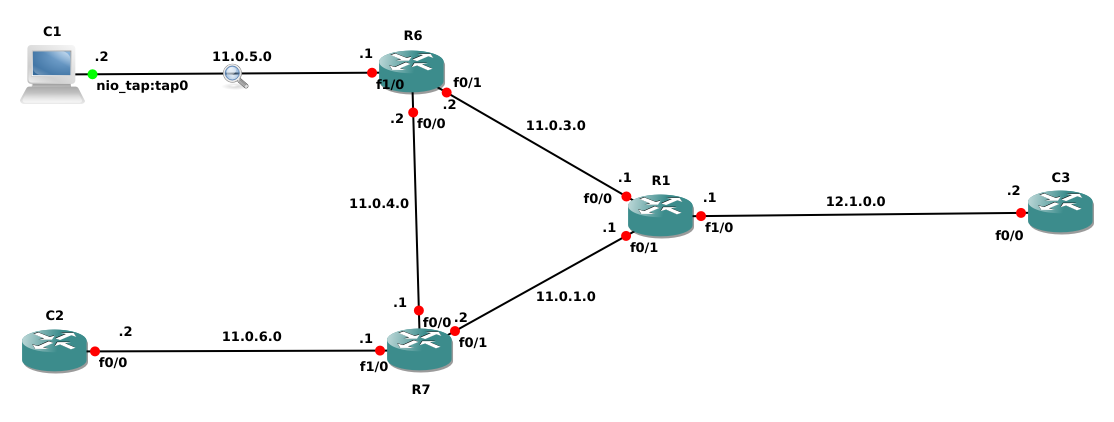
\includegraphics[scale=0.4]{Images/topology1.png}
\caption{Multicast - Topologia de la xarxa a efectuar l'exercici}
\end{center}
\end{figure}
Per a la realització de aquest exercici utilitzarem encaminadors \textbf{Cisco c7200}
\subsection{Principals problemes de configuració i com ho hem solucionat}
Primer de tot, hem configurat la topologia utilitzant encaminadors amb multicast ip routing activat i posant les seves interfícies a pim dense mode. Els 3 encaminadors, C1,C2 i C3, els hem afegit al grup 111 de multicast i hem comprovat la seva connectivitat.
\\\\
\begin{figure}[H]
\begin{center}
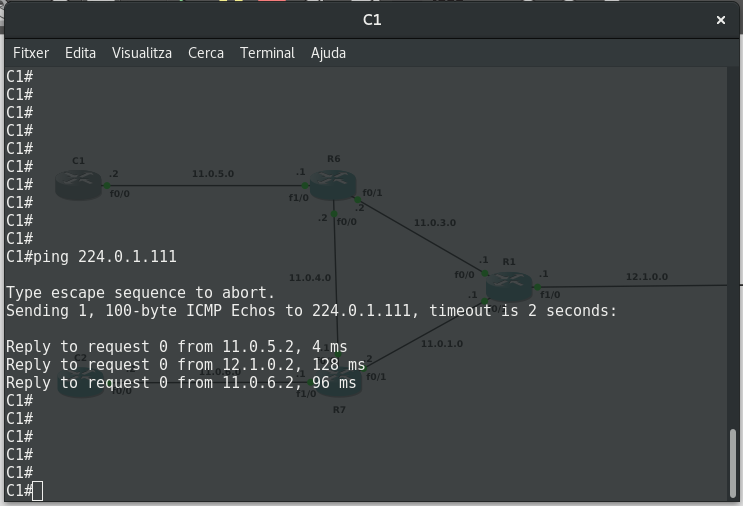
\includegraphics[scale=0.34]{Images/1aPartC1.png}
\caption{Multicast - Encaminador C1}
\end{center}
\end{figure}
\begin{figure}[H]
\begin{center}
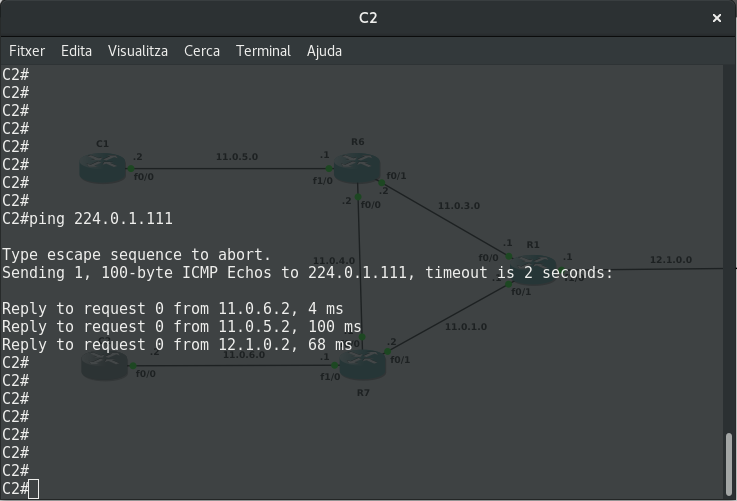
\includegraphics[scale=0.34]{Images/1aPartC2.png}
\caption{Multicast - Encaminador C2}
\end{center}
\end{figure}
\begin{figure}[H]
\begin{center}
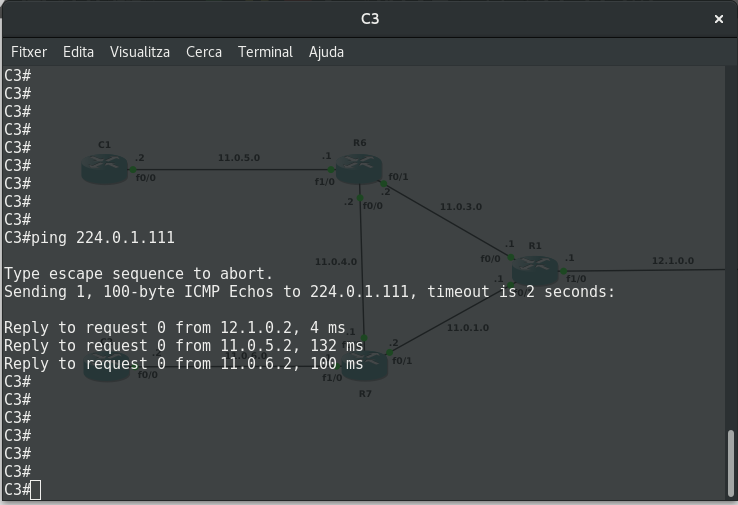
\includegraphics[scale=0.34]{Images/1aPartC3.png}
\caption{Multicast - Encaminador C3}
\end{center}
\end{figure}
Quan ens ha funcionat això, hem canviat el encaminador C1, per una interfície tap del nostre ordinador. Aquí hem començat a tindre problemes. Ens hem llegit el document que ens vas enviar i hem descarregat el smcroute per poder configurar multicast dense mode. El problema és que només podíem veure des de la interfície el propi ping multicast, i pensàvem que no acabava de funcionar, però hem pogut comprovar qe si fem \textbf{ping 224.0.1.111 -t10} podem veure les IPs duplicades i així apareixen les dels altres encaminadors.
\\\\
A continuació, posem una captura d'aquests paquets i les comandes per poder crear la interfície.
\begin{figure}[H]
\begin{lstlisting}[style=C]
echo "Creating Tap0"
sudo tunctl -t tap0 -u cesar
sudo ip link set tap0 up
sudo ip add add 11.0.5.2/24 dev tap0
echo "Created Tap0"

echo "configurant rutes i multicast_tap0"
sudo route add -net 11.0.5.0 netmask 255.255.255.0 dev tap0 
sudo route add -net 224.0.0.0 netmask 224.0.0.0 dev tap0
sudo route add -net 12.1.0.0 netmask 255.255.255.0 gw 11.0.5.1
sudo route add -net 11.0.6.0 netmask 255.255.255.0 gw 11.0.5.1
sudo sysctl net.ipv4.icmp_echo_ignore_broadcasts=0
sudo smcroute-0.92/bin/smcroute -d
sudo smcroute-0.92/bin/smcroute -j tap0 224.0.1.111
echo "rutes OK" 
echo "multicast OK"

ping 224.0.1.111 -t10
\end{lstlisting}
\caption{Multicast - Comandes per executar correctament multicast amb interfície}
\end{figure}
\begin{figure}[H]
\begin{center}
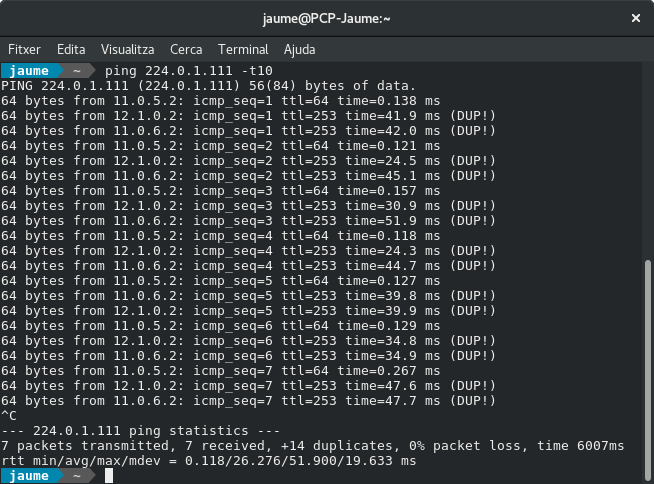
\includegraphics[scale=0.5]{Images/1aPartTap.png}
\caption{Multicast - Encaminador C1 amb interfície Tap0}
\end{center}
\end{figure}
\newpage
\section{Túnels GRE}
Túnel és una tècnica que consisteix en encapsular un protocol de xarxa sobre un altre, creant així un túnel d'informació dins d'una xarxa.  Aquesta tècnica acostuma a ser utilitzada per transportar un protocol determinat a través d'una xarxa que, en condicions normals, no seria possible o també s'utilitza per crear xarxes privades virtuals.\\\\
En el nostre cas, per la realització de la pràctica utilitzarem túnels GRE.
\\\\
\textbf{Generic Routing Encapsulation (GRE)} és un protocol de túnel desenvolupat per \textit{Cisco Systems} que té la capacitat de encapsular una gran varietat de protocols de capa de xarxa a l'interior d'enllaços virtuals de punt a punt a través del protocol d'Internet.
\subsection{Topologia de la xarxa}
\begin{figure}[H]
\begin{center}
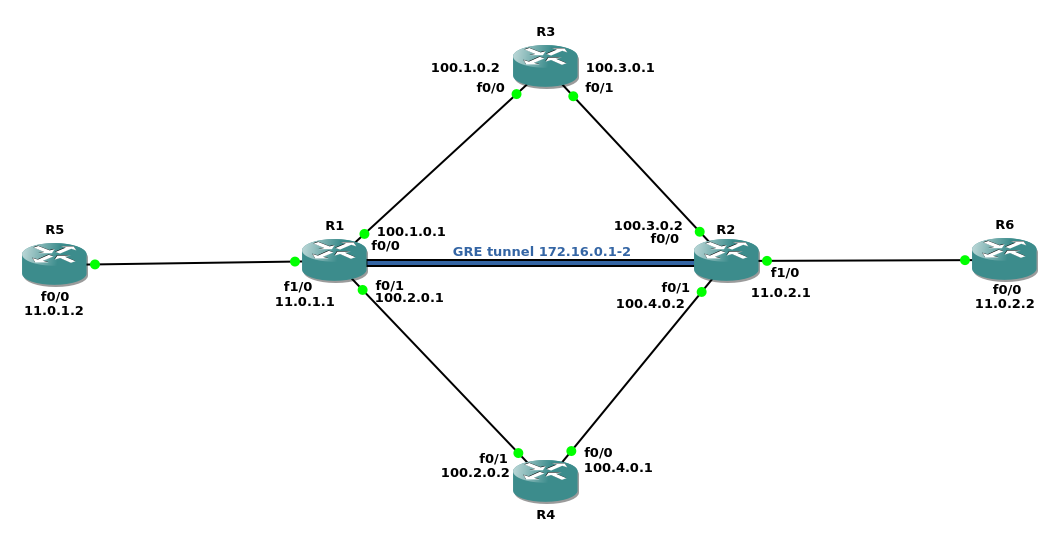
\includegraphics[scale=0.4]{Images/topology2.png}
\caption{Túnels GRE - Topologia de la xarxa a efectuar l'exercici}
\end{center}
\end{figure}
Per a la realització de aquest exercici utilitzarem encaminadors \textbf{Cisco c7200}
\subsection{Per quins encaminadors passa el paquet \emph{ping} ?}
\emph{Feu un ping de la interfície \textbf{11.0.1.2} al \textbf{11.0.2.2} i comproveu per quins encaminadors passa el paquet.}
\begin{figure}[H]
\begin{center}
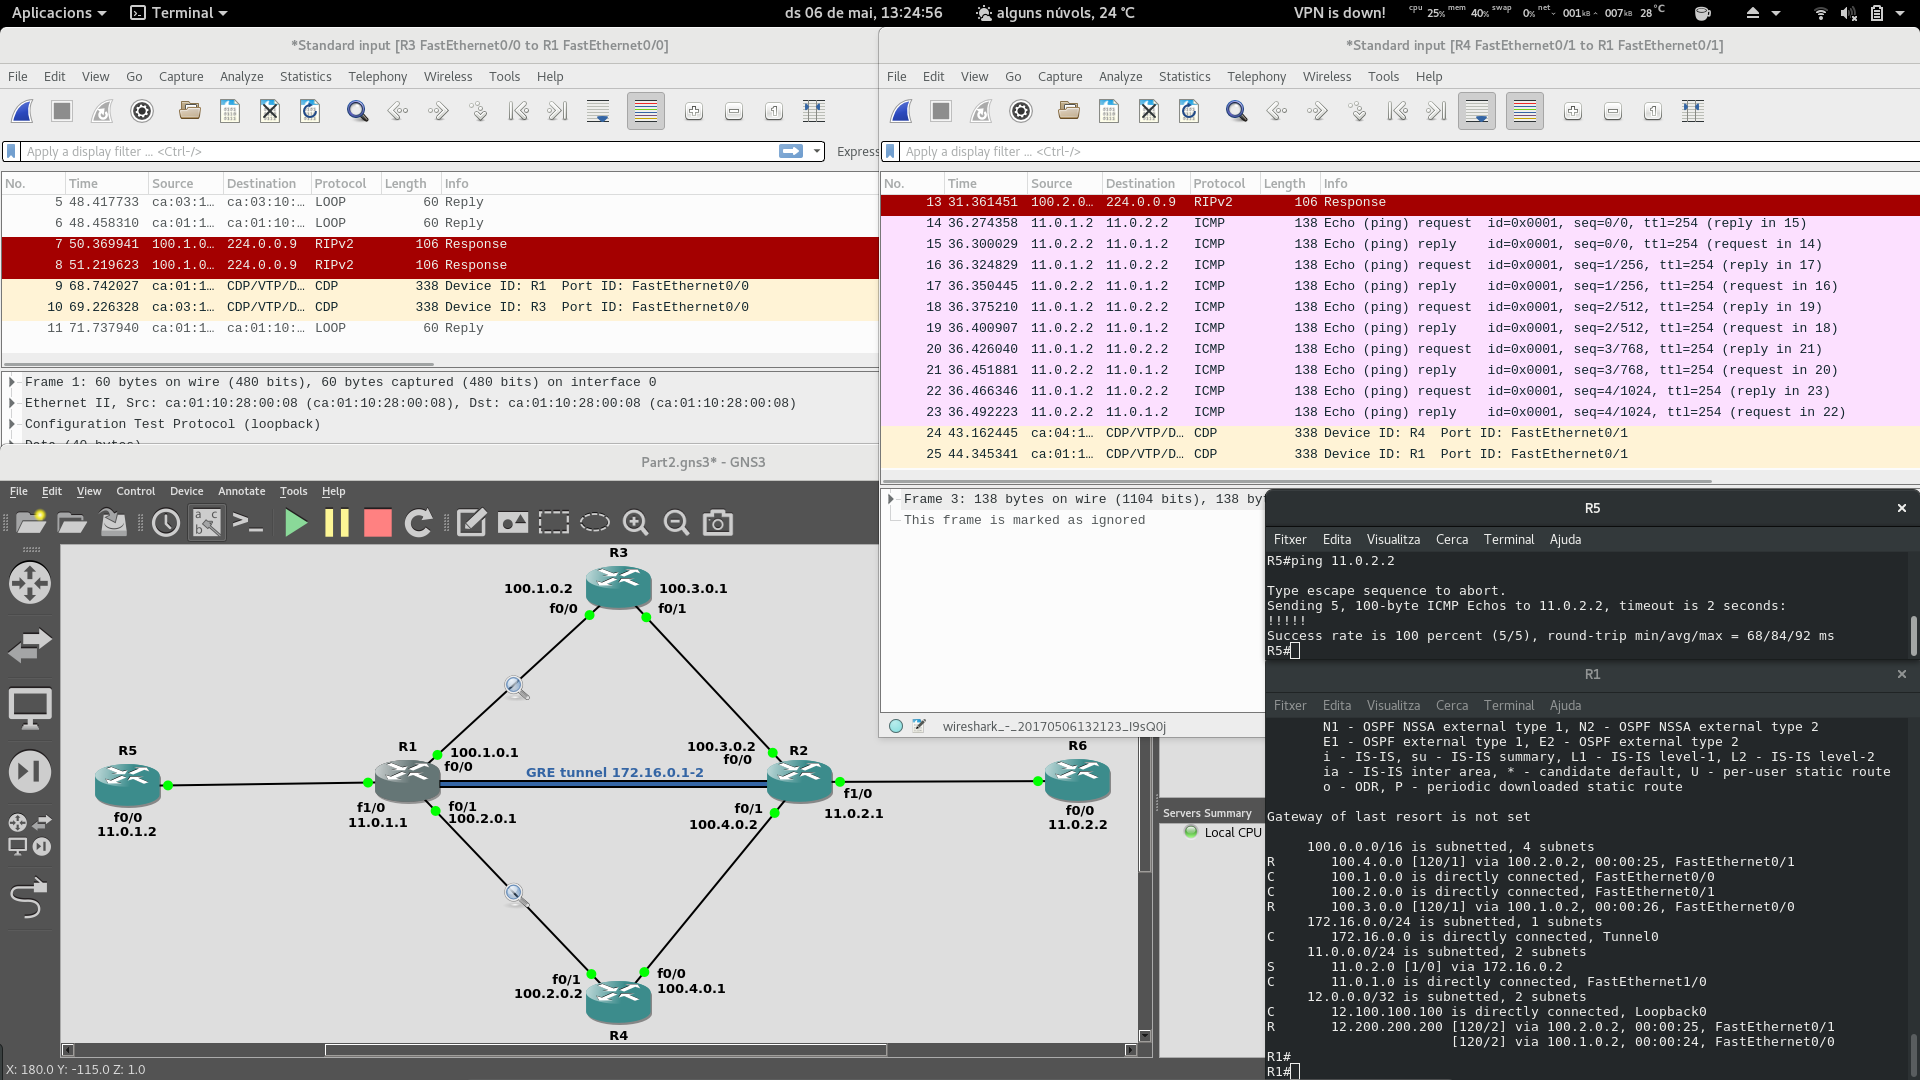
\includegraphics[scale=0.24]{Images/part2Ex1.png}
\caption{Paquet ping a la interfície 11.0.2.2}
\end{center}
\end{figure}
Com podem veure en la captura superior, podem veure que el paquet ICMP passa per el els encaminadors \textbf{R1, R4 i R2}.
\\\\
\emph{Atureu el encaminador que travessa el paquet i comproveu que continueu tenint ping. Quant de temps ha de passar? Perquè?}\\\\
Després de comprovar que el encaminador R4 és travessat per el paquet ICMP, l'hem aturat i després de esperar un temps hem comprovat que tot i tenir el encaminador R4 aturat, teníem connectivitat per l'encaminador R3. Hem hagut d'esperar 240 segons degut a que és el temps que triga el protocol RIP a comprovar que la xarxa està caiguda i eliminar-lo de la llista de rutes del encaminador (Flush Time), i per tant no utilitza l'altra ruta fins treure la ruta d'aquell encaminador.
\subsection{Principals problemes de configuració i com els hem resolt}
En aquest exercici, els problemes de configuració han sigut mínims, degut a que ja sabíem implementar el protocol d'encaminament de l'altra pràctica i la creació del túnel no ens va suposar un gran problema. Un petit problema que vam tindre va ser que la xarxa \textbf{12.X.X.X} que havíem de canviar,no vam canviar les xarxes \textbf{12.100.100.100 i 12.200.200.200} i per tant, no havia manera de que hi hagués connectivitat fins que vam posar aquestes dues xarxes i ja va funcionar tot correctament.
\newpage
\section{Multicast en túnels GRE}
En molts escenaris de xarxa, és vol configurar la xarxa per utilitzar els túnels GRE per enviar la multidifusió independent de protocol (PIM) i el trànsit Multicast entre el Routers. Típicament, això passa en l'origen de la multi-difusió i el receptor els quals no estan físicament connectats, sinó que estan separats per Internet.En aquests escenaris de xarxa, configurar un túnel a través d'internet amb el PIM habilitat transporta els paquets de multidifusió cap al receptor.
\subsection{Topologia de la xarxa}
\begin{figure}[H]
\begin{center}
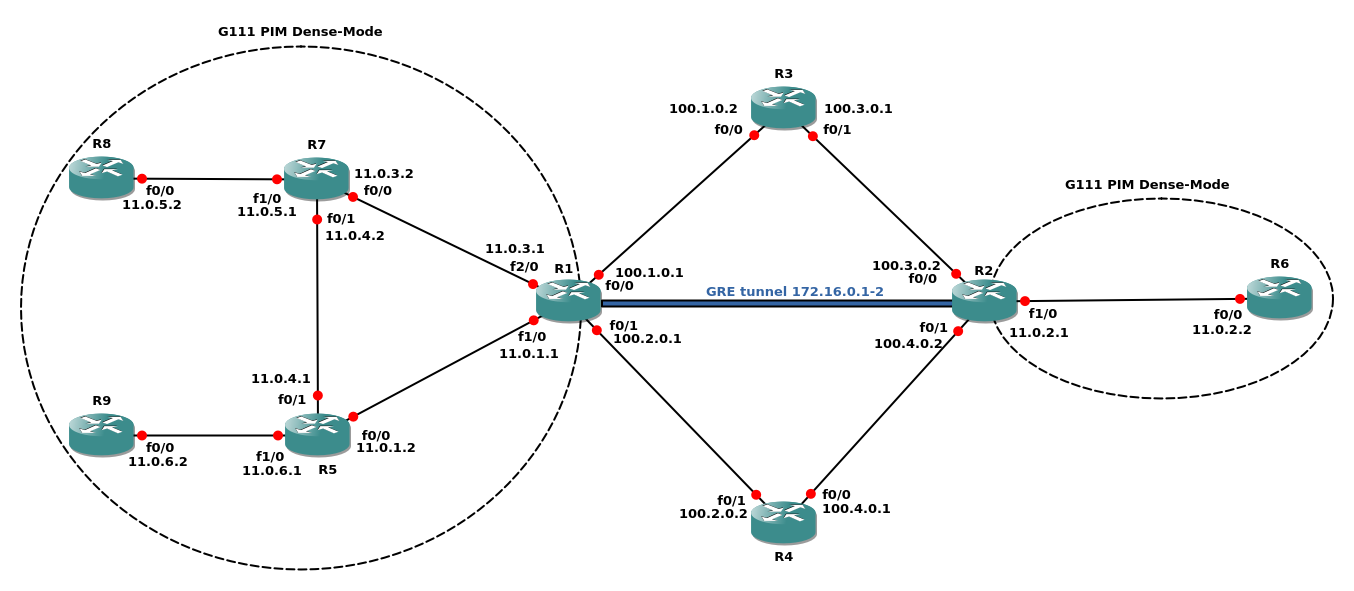
\includegraphics[scale=0.4]{Images/topology3.png}
\caption{Múlticast en túnels GRE - Topologia de la xarxa a efectuar l'exercici}
\end{center}
\end{figure}
Per a la realització de aquest exercici utilitzarem encaminadors \textbf{Cisco c7200}
\subsection{Captures de pantalla}
\begin{figure}[H]
\begin{center}
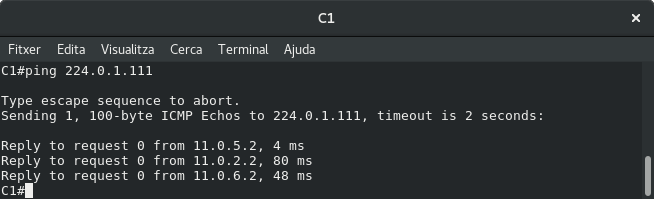
\includegraphics[scale=0.4]{Images/C1.png}
\caption{Múlticast en túnels GRE - Router C1}
\end{center}
\end{figure}
\begin{figure}[H]
\begin{center}
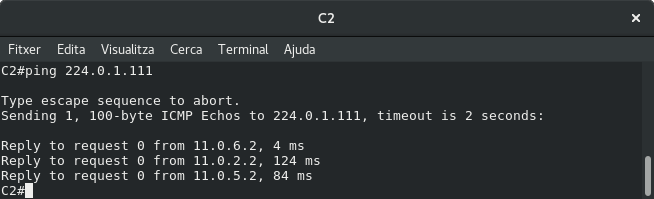
\includegraphics[scale=0.4]{Images/C2.png}
\caption{Múlticast en túnels GRE - Router C2}
\end{center}
\end{figure}
\begin{figure}[H]
\begin{center}
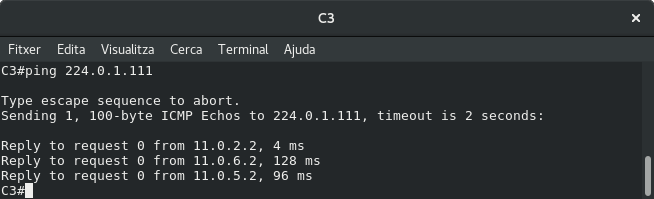
\includegraphics[scale=0.4]{Images/C3.png}
\caption{Múlticast en túnels GRE - Router C3}
\end{center}
\end{figure}
\begin{figure}[H]
\begin{center}
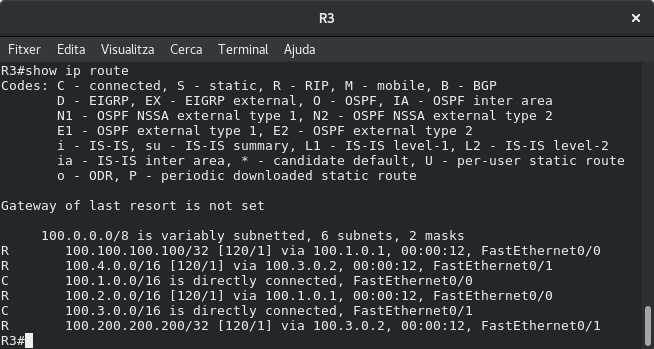
\includegraphics[scale=0.4]{Images/R3.png}
\caption{Múlticast en túnels GRE - Router R3}
\end{center}
\end{figure}
\begin{figure}[H]
\begin{center}
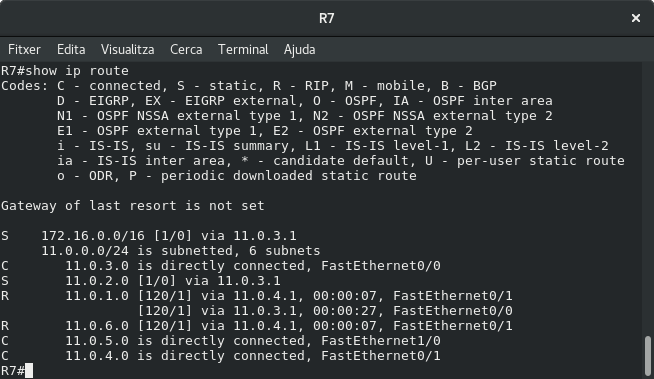
\includegraphics[scale=0.4]{Images/R7.png}
\caption{Múlticast en túnels GRE - Router R7}
\end{center}
\end{figure}
\subsection{Principals problemes de configuració i com els hem resolt}
Després de tindre l'exercici 2 configurat correctament i funcionant, hem adaptat la topologia que teníem a la de l'exercici. Quan hem configurat les interfícies, hem posat tots els encaminadors en mode multicast i hem habilitat les seves interfícies per transit multicast PIM dense mode. Finalment hem configurat els encaminador C1, C2 i C3 com a encaminadors del grup G111 i ho hem provat. El problema principal ha sigut que ens els encaminadors R7,R5,R4 i R3 hi havien rutes que no hi havien de ser. Això ho hem solucionat afegint rutes estàtiques i utilitzant les \href{http://www.ciscopress.com/articles/article.asp?p=2273507&seqNum=10}{llistes de distribució}.
\end{document}
              
